\documentclass{beamer}

\mode<presentation> {
\usetheme{Boadilla}
\usecolortheme{whale}
}

\newcommand{\pp}{\partial}
\newcommand{\CC}{\mathbb{C}}
\newcommand{\CCC}{\mathcal{C}}
\newcommand{\NN}{\mathbb{N}}
\newcommand{\RR}{\mathbb{R}}
\newcommand{\QQ}{\mathbb{Q}}
\newcommand{\ZZ}{\mathbb{Z}}
\newcommand{\FF}{\mathbb{F}}
\newcommand{\PP}{\mathcal{P}}
\newcommand{\DD}{\mathcal{D}}
\newcommand{\ee}{\mathrm{e}}
\newcommand{\HH}{\mathcal{H}}
\newcommand{\C}{\mathrm{C}}
\newcommand{\HHH}{\mathrm{H}}
\newcommand{\II}{\mathcal{I}}
\newcommand{\III}{\mathrm{I}}
\newcommand{\LL}{\mathcal{L}}
\newcommand{\p}{\rho}
\newcommand{\tp}{\tilde{\rho}}
\newcommand{\e}{\varepsilon}
\newcommand{\OO}{\Omega}


\usepackage{tikz}
\usetikzlibrary{shapes, tikzmark}
\tikzset{every tikzmarknode/.style={draw=red, thick, inner sep=2pt}}

\usepackage{graphicx} % Allows including images
\usepackage{animate}
\usepackage{algorithm,algorithmic}
\usepackage{multicol}
\usepackage{booktabs} % Allows the use of \toprule, \midrule and \bottomrule in tables
\usepackage{mathtools}

\title[]{Responsive optimal design with stimulus as design and state variable} % The short title appears at the bottom of every slide, the full title is only on the title page

\author{Jamal Shabani} % Your name
\institute[] % Your institution as it will appear on the bottom of every slide, may be shorthand to save space
{
    McMaster University \\ % Your institution for the title page
    \medskip
    \textit{PhD Defence} % Your email address
}
\date{September 05, 2024} % Date, can be changed to a custom date
\begin{document}

\begin{frame}
\titlepage % Print the title page as the first slide
\end{frame}

\AtBeginSection[]
{
    \begin{frame}
        \frametitle{Outline}
        \tableofcontents[currentsection]
    \end{frame}
}

%%%%%%%%% Begin of SECTION 1 %%%%%%%
\section{Introduction}
\subsection{Responsive optimal design}
\begin{frame}{Responsive optimal design}
\begin{itemize}
    \item Optimal design deals with finding the allocation of several materials in order to enhance the performance of a structure.
    \begin{figure}[h]
        \centering
        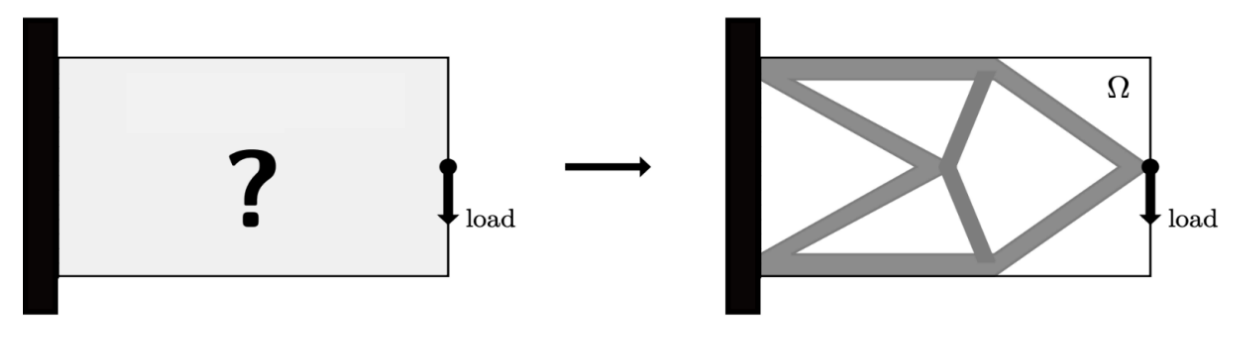
\includegraphics[width=0.6\textwidth]{figures/minimum.png}
    \end{figure}
    \item Responsive materials are those materials whose properties can changed by external stimulus.
    \item Examples of responsive materials
    \begin{enumerate}
        \item Shape Memory Alloy (SMA)
        \item Thermoelastic material
    \end{enumerate} 
    \item Three design materials \emph{i.e} {\bf void/holes, non-responsive and responsive}
    \item \textcolor{red}{\bf Goal:} Optimal allocation of ({\bf void/holes, non-responsive and responsive}) 
    materials and the {\bf stimulus} or {\bf stimulus control} that optimizes some general objective.
\end{itemize}
\end{frame} 
%%%%%%%%% End of SECTION 1 %%%%%%%

%%%%%%%%% Begin of SECTION 2 %%%%%%%
\section{Responsive optimal design with stimulus as a design variable}
\subsection{Problem statement}
\begin{frame}{Problem statement}
\begin{itemize}
    \item Consider a ground domain $\Omega \in \RR^d,d=2,3$ subject to boundary force 
    $f$ on a part $\Gamma_N \in \partial \OO$ of its boundary and clamped 
    on $\Gamma_D \in \partial \OO.$
    \bigskip

    \item Let $\chi_v, \chi_s,$ and $\chi_r$ be a characteristic functions such that 
        \[ \chi_{v,s,r}(x)= \begin{cases} 
            1 & x \in \text{Void, Non-responsive, Responsive,}\\
            0 & x \notin \text{Void, Non-responsive, Responsive.}
        \end{cases}
        \]
    \bigskip
    \item We want the constraints $$\chi_v(x)+\chi_s(x)+\chi_r(x)=1,\forall {x \in \OO},$$
    $$\int_\OO \chi_{v,s,r}\, dx = \theta_{v,s,r}|\OO| \text{ such that }\theta_v + \theta_s + \theta_r = 1.$$
    \bigskip
    \item Design variable $\Phi=[\chi_v,\chi_s,\chi_r]^T.$
\end{itemize}
\end{frame}


\begin{frame}{Problem statement}
    \begin{itemize}
        \item Consider the constitutive law
        $$\sigma(u_j) = \sum_{i=\{v,s,r\}}\chi_i\mathbb{C}_i \left(\ee(u_j) - \beta_i s_j\mathrm{I}_d\right)$$
        where $\mathbb{C}_i$ denotes the Hooke's law for material $i$ and $\ee(u_j)=\frac{1}{2}(\nabla u_j + (\nabla u_j)^T)$ 
        is the linearized strain associated to a displacement field $u_j$.
        \bigskip
        \item $\beta_i$ is a given parameter such that $\beta_v=\beta_s=0, \beta_r=1$, $s_j \in [-1,1]$ is the stimulus associated with $u_j$ and $\mathrm{I}_d$ is $d \times d$ identity matrix.
        \bigskip
        \item Define the least square objective function
        \begin{equation}
            \label{eq:objectiveFunctionNoPerimeter}
            \mathcal{I}(u_1,\dots,u_n) := \sum_{j=1}^n\frac{1}{2}\int_{\OO_0} |u_j(x) - \bar{u}_j(x)|^2\, dx,
        \end{equation}
        where $\bar{u}_1,\ldots,\bar{u}_n$ are the target displacements.
    \end{itemize}
\end{frame}

\begin{frame}{Problem statement}
    \begin{itemize}
        \item The displacement fields $u_j \in V$, $1 \le j \le n$,  satisfy the weak form of the linearized elasticity system 
        \begin{equation}
            \label{eq:stateSharpWeak}
            \sum_{i=\{v,s,r\}}\int_{\OO}\chi_i \mathbb{C}_i\left(\ee(u_j) - \beta_i s_j\mathrm{I}_d\right)\cdot \ee(v)\, dx = 0,\forall v \in V,
        \end{equation}
        where 
        \begin{equation}\label{eq:sobolevSpace}
            V:= \left\{ v \in H^1(\Omega);\, v = 0 \text{ on } \Gamma_D \right\}.
        \end{equation}
        \item Mathematically, the responsive optimal design problem reads as
        \begin{equation}\label{eq:generalOptimalDesignProblem1}
        \begin{dcases}
        \begin{aligned}
              &\inf_{(\Phi,\mathrm{s})}\;\; \II(u_1,u_2,\ldots,u_n)\\
             &u_j\text{ satisfies the state equation }(\ref{eq:stateSharpWeak})
        \end{aligned}
        \end{dcases}
        \end{equation}
        where $\mathrm{s}:=(s_1, \dots , s_n).$
        \smallskip
        \item The problem $(\ref{eq:generalOptimalDesignProblem1})$ is ill-posed
        \smallskip
        \item How to make the problem $(\ref{eq:generalOptimalDesignProblem1})$ well-posed?
        \smallskip
        \begin{itemize}
           \item Perimeter penalization
        \end{itemize}
    \end{itemize}
\end{frame}

\begin{frame}{Problem statement}
    \begin{itemize}
        \item Let $\mathrm{D}=(D_v,D_s,D_r)$ be a partition of the domain $\OO$ such that $\chi_{v,s,r}=\chi_{D_{v,s,r}}$ and define
        \begin{equation}
            \label{eq:defP}
            \mathcal{P}(\mathrm{\chi}) := \frac12 \sum_{i, j=\{v,s,r\}, i \neq j} \mathcal{H}^{d-1}\left(\partial D_i \cap \partial D_j \cap \Omega\right),
        \end{equation} 
        where $\mathcal{H}^{d-1}$ denotes the $d-1$ dimensional Hausdorff
        \bigskip
        \item Given a small regularization parameter $\alpha > 0$, we study the problem
        \begin{equation}\label{eq:perimeter}
            \inf_{(\Phi,\mathrm{s})}\;\; \mathcal{I}(u_1,\dots,u_n) + \alpha\mathcal{P}(\chi).
        \end{equation}
        \bigskip
        \item \textcolor{red}{\bf Problem:} It is not easy to implement $(\ref{eq:perimeter}).$
    \end{itemize}
\end{frame}

\subsection{The phase field approach  to optimal design}
\begin{frame}{The phase field approach  to optimal design}
\begin{itemize}
    \item We introduce designs of the form $\p = (\p_v,\p_s,\p_r),$
    where each $\p_v,\p_s,\p_r \in H^1(\OO;[0,1])$ is a smooth continuous density function.

    \item For any $\varepsilon>0,$ define the vector-valued Modica-Mortola functional
    \begin{equation}\label{vector-valued-mm}
        \PP_{\varepsilon}(\p)= \int_{\OO}\frac{W(\rho)}{\e}+\e|D\rho|^2\; dx.
    \end{equation}
    \item $W(\p)$ is a non-negative multiple-well potential function vanishing only at three points $(1,0,0),(0,1,0)\text{ and }(0,0,1)$
    and satisfying
    \begin{align*}
        \label{eq:normalizationW}
        d_{ij}:= \inf \Biggl\{\int_0^1 W^{1/2}(\gamma(t))|\gamma'(t)|\,&dt; \gamma \in C^{1}((0,1);\RR^m),\\
        &\gamma(0)=\p_i,\gamma(1)=\p_j \Biggr\} = 1
    \end{align*}
\end{itemize}
\end{frame}

\begin{frame}{The phase field approach  to optimal design}
    \begin{itemize}
        \item The space of admissible designs $\mathcal{D}_{\rho}$ and stimuli $\mathcal{S}$
        \begin{equation*}
            \mathcal{D}_\rho:=\Bigl\{\p \in \left[H^1(\OO;[0,1])\right]^3,
            \sum_{i=\{v,s,r\}}\p_i=1,\int_\OO \rho_{v,s,r}\, dx = \theta_{v,s,r}|\OO|\Bigr\},
        \end{equation*}
        \begin{equation*}\label{eq:defS}
            \mathcal{S}:= L^1\left(\OO,[-1,1]^n\right).
        \end{equation*}
        \item The phase field  regularization of~\eqref{eq:perimeter} is then
        \begin{equation}\label{eq:phaseFieldRegularization}
            \inf_{(\rho,\mathrm{s}) \in \mathcal{D_\rho} \times \mathcal{S}} \mathcal{I}(u_1,\dots,u_n) + \alpha\mathcal{P}_\e(\rho).
        \end{equation}
        where $u_j \in V$ satisfies the weak formulation
        \begin{equation}
            \label{eq:statePFWeak}
            \sum_{i=\{v,s,r\}}\int_\OO a(\p_i)\mathbb{C}_i\left(\ee(u_j)-\beta_i s_j\mathrm{I}_d\right)\cdot \ee(v)\, dx = 0\ \forall v \in V,\  1 \le j \le n
        \end{equation} and $a$ is a continuous function such that $a(0)=0$ and $a(1)=1.$
    \end{itemize}
\end{frame}

\subsection{Existence of solutions}
\begin{frame}{Existence of solutions}
    \begin{itemize}
        \item Define $\widetilde{\mathcal{I}}(\rho,\mathrm{s}) = \mathcal{I}\left(u_1(\rho,s_1), \dots, u_n(\rho,s_n)\right).$
        \item Consider the problem
        $$\mathop{\arg \min}\limits_{(\p,\mathrm{s}) \in \mathcal{D_\rho} \times \mathcal{S}}\; \widetilde{\mathcal{I}}(\rho,\mathrm{s})+\widetilde{\PP}_{\varepsilon}(\p, \mathrm{s}) \stackrel{\Gamma}{\longrightarrow} \mathop{\arg \min}\limits_{(\p,\mathrm{s}) \in \mathcal{D_\rho} \times \mathcal{S}}\; \widetilde{\mathcal{I}}(\rho,\mathrm{s})+\widetilde{\PP}(\p,\mathrm{s})$$
        where \begin{equation*}
            \widetilde{\mathcal{P}}_\e(\p,\mathrm{s}) := \begin{cases}
                \mathcal{P}_\e(\p) & \text{ if } (\p,\mathrm{s}) \in \mathcal{D}_\p\times\mathcal{S}\\
                +\infty & \text{ otherwise,}
            \end{cases}
        \end{equation*}
        \item $\Gamma-$convergence is stable under continuous perturbation.
        \item It is enough to prove continuity of $\widetilde{\mathcal{I}}(\rho,\mathrm{s})$ w.r.t to $\p$ and $\mathrm{s}.$
        \begin{theorem}[Fundamental Theorem of $\Gamma-$Convergence]
            Let $X$ be a topological space. Let $(F_n)$ be an equi-coercive sequence of functions and let $F_n$ $\Gamma-$converges to
            $F$ in $X$, then the minimizers of $F_n$ converge to a minimizer of $F.$
            
        \end{theorem}
    \end{itemize}
\end{frame}


\begin{frame}{Existence of solutions}
    \begin{lemma}[1]
        \label{lem:equicoercivity}
        Let $(\rho,\mathrm{s}) \in \mathcal{D}_{\p}\times \mathcal{S}$ 
        and $k_1,k_2>0$ be such that for any $1 \le i \le 3$ and for 
        any $\Psi \in \mathrm{M}^{d\times d}_\mathrm{sym},$ we have
            $k_1 \Psi\cdot \Psi \le \mathbb{C}_i \Psi\cdot \Psi \le k_2 \Psi\cdot \Psi.$
        There exists $C>0$ such that if $u_j \in V$ satisfies~\eqref{eq:stateSharpWeak}, then
            $$\|u_j\|_{H^1(\Omega)} \le C ,\  1 \le j \le n.$$
    \end{lemma}
    \begin{proof}
        By taking $u_j \in V$ as the test function, linearized weak form~\eqref{eq:statePFWeak} becomes,
        \begin{equation}
            \sum_{i=\{v,s,r\}}\int_{\OO}a(\p_i) \mathbb{C}_i\ee(u_j)\cdot \ee(u_j)\, dx = \sum_{i=\{v,s,r\}}\int_{\OO}a(\p_i)\beta_i s_j\mathbb{C}_i\mathrm{I}_d\cdot \ee(u_j)\, dx,
        \end{equation}
    \end{proof}
\end{frame}

\begin{frame}{Existence of solutions}
    \begin{proof}[\proofname\ (Cont.)]
        We get,
        $$
            k_1\|e(u_j)\|_{L^2}^2 \leq \left\|\sum_{i=\{v,s,r\}}a(\p_i)\beta_i s_j\mathbb{C}_i\mathrm{I}_d\right\|_{L^2 }\|e(u_j)\|_{L^2},
        $$
        and hence $$\|e(u_j)\|_{L^2} \leq M.$$ By Korn's inequality, we have that the solution $u_j$ is bounded
        $$C\|u_j\|_{H^1} \leq \|e(u_j)\|_{L^2} \leq M \implies \|u_j\|_{H^1} \leq M.$$
    \end{proof}
\end{frame}

\begin{frame}
    \begin{theorem}[Continuity of displacements $\implies$ continuity of $\widetilde{\mathcal{I}}(\rho,\mathrm{s})$]
        Consider a sequence $(\p_\e,\mathrm{s}_\e) \in \mathcal{D}_\p \times S$ of designs and stimuli 
        such that $\p_\e \to \p,$ in $\left[L^1(\Omega)\right]^3$ 
        and $\mathrm{s}_\e \rightharpoonup \mathrm{s}$ 
        in  $\left[L^2(\Omega)\right]^n$. Let $u_\e = (u_{1,\e},\dots,u_{n,\e})$ 
        (resp. $u = (u_1,\dots,u_n)$) be the equilibrium displacements associated 
        with $(\p_\e,\mathrm{s}_\e)$ (resp. $(\p,\mathrm{s})$).
        Then if the $\mathbb{C}_i$ satisfies the hypotheses of Lemma~\ref{lem:equicoercivity}, $u_\e \to u$ in $\left[L^2(\OO)\right]^n$
        and $\widetilde{\mathcal{I}}(\rho_{\e},\mathrm{s}_{\e}) \longrightarrow \widetilde{\mathcal{I}}(\rho,\mathrm{s}).$
        \end{theorem}
    \begin{proof}
        For each $(\p_{\e},\mathrm{s}_{\e})$ we can find sequence $u_{\e}$ 
        such that $u_{\e}$ is the solution of the linearized elasticity PDE 
        associated with $(\p_{\e},\mathrm{s}_{\e}).$ Since $u_{\e}$ is uniformly bounded 
        in $H^1$ we can extract a convergent subsequence $u_{{\e}_n}$ converging 
        weakly to some $u \in H^1.$  
        Recalling
        $$\widetilde{\mathcal{I}}(\rho_{\e},\mathrm{s}_{\e}) = \mathcal{I}\left(u_{1,\e}(\rho_{\e},s_{1,\e}), \dots, u_{n,\e}(\rho_{\e},s_{n,\e})\right),$$
        
    \end{proof}
\end{frame}

\begin{frame}
    \begin{proof}[\proofname\ (Cont.)]
        and since $u_{{\e}_n} \rightarrow u$ strongly in $L^2$ we can pass the limit inside to get
        \begin{align*}
            \widetilde{\mathcal{I}}(\rho_{\e},\mathrm{s}_{\e}) &= \mathcal{I}\left(u_{1,\e}(\rho_{\e},s_{1,\e}), \dots, u_{n,\e}(\rho_{\e},s_{n,\e})\right)\\
            &\rightarrow \mathcal{I}\left(u_{1}(\rho,s_{1}), \dots, u_{n}(\rho,s_{n})\right)\\
            &= \widetilde{\mathcal{I}}(\rho,\mathrm{s}).
        \end{align*}
    \end{proof}
    \begin{block}{Note}
        The proof above assumes the minimizing sequence $(\p_{\varepsilon}, \mathrm{s}_{\varepsilon})$ is compact.
    \end{block}
\end{frame}

\subsection{Numerical implementation}
\begin{frame}{Numerical implementation}
    \begin{itemize}
        \item The constraint $\p_v+\p_s+\p_r=1 \implies \p_v= 1 - \p_s - \p_r$ 
        and introduce $\tp = (\p_s,\p_r).$
        \item We add pernalties $Q(\tp,\mathrm{s})$ and $V_C(\tp)$
        where $$Q(\tp,\mathrm{s})=\int_{\OO}(\p_v^2+\p_s^2)s^2\;dx=\int_{\OO}((1-\p_s-\p_r)^2+\p_s^2)s^2\;dx$$ and 
        $$V_C(\tp) = \nu_s\int_{\OO}\p_s\;dx + \nu_r\int_{\OO}\p_r\,dx.$$
        \item We consider the problem:
        \begin{equation}
            \begin{dcases}
            \begin{aligned}
                &\min_{(\p,\mathrm{s}) \in \mathcal{D}_{\p} \times \mathcal{S}}\;\; \sum_{j=1}^n\frac{1}{2}\int_{\OO_0}|u_j-\bar{u}_j|^2\;dx + \alpha\PP_{\e}(\tp,\mathrm{s}) + Q(\tp,\mathrm{s}) + V_C(\tp)\\
                &u_j\text{ satisfies the weak form }(\ref{eq:statePFWeak})
            \end{aligned}
            \end{dcases}
        \end{equation}
    \end{itemize}
\end{frame}

\begin{frame}{Numerical implementation}
    \begin{itemize}
        \item We apply the adjoint method to compute the derivative of the objective function
        \bigskip
        \item By collecting all terms explicitly depending on $s \implies$ 
        closed form of an optimal stimulus.
        \bigskip
        \item We tested two different numerical approaches.
        \bigskip
        \begin{enumerate}
            \item {\bf Staggered} approach $\implies$ minimize w.r.t $\tp$ only and update $s$ explicitly.
            \item {\bf Monolithic} approach $\implies$ minimize w.r.t $\tp$ and $s$ simultaneously.
        \end{enumerate}
        \bigskip
        \item Our numerical implementation uses Firedrake and TAO
    \end{itemize}
\end{frame}

\subsection{Numerical results}
\begin{frame}{Numerical results}
    \begin{itemize}
        \item Target displacement $\bar{u}=(0,1).$
    \end{itemize}
    \begin{figure}[H]
        \begin{multicols}{2}
            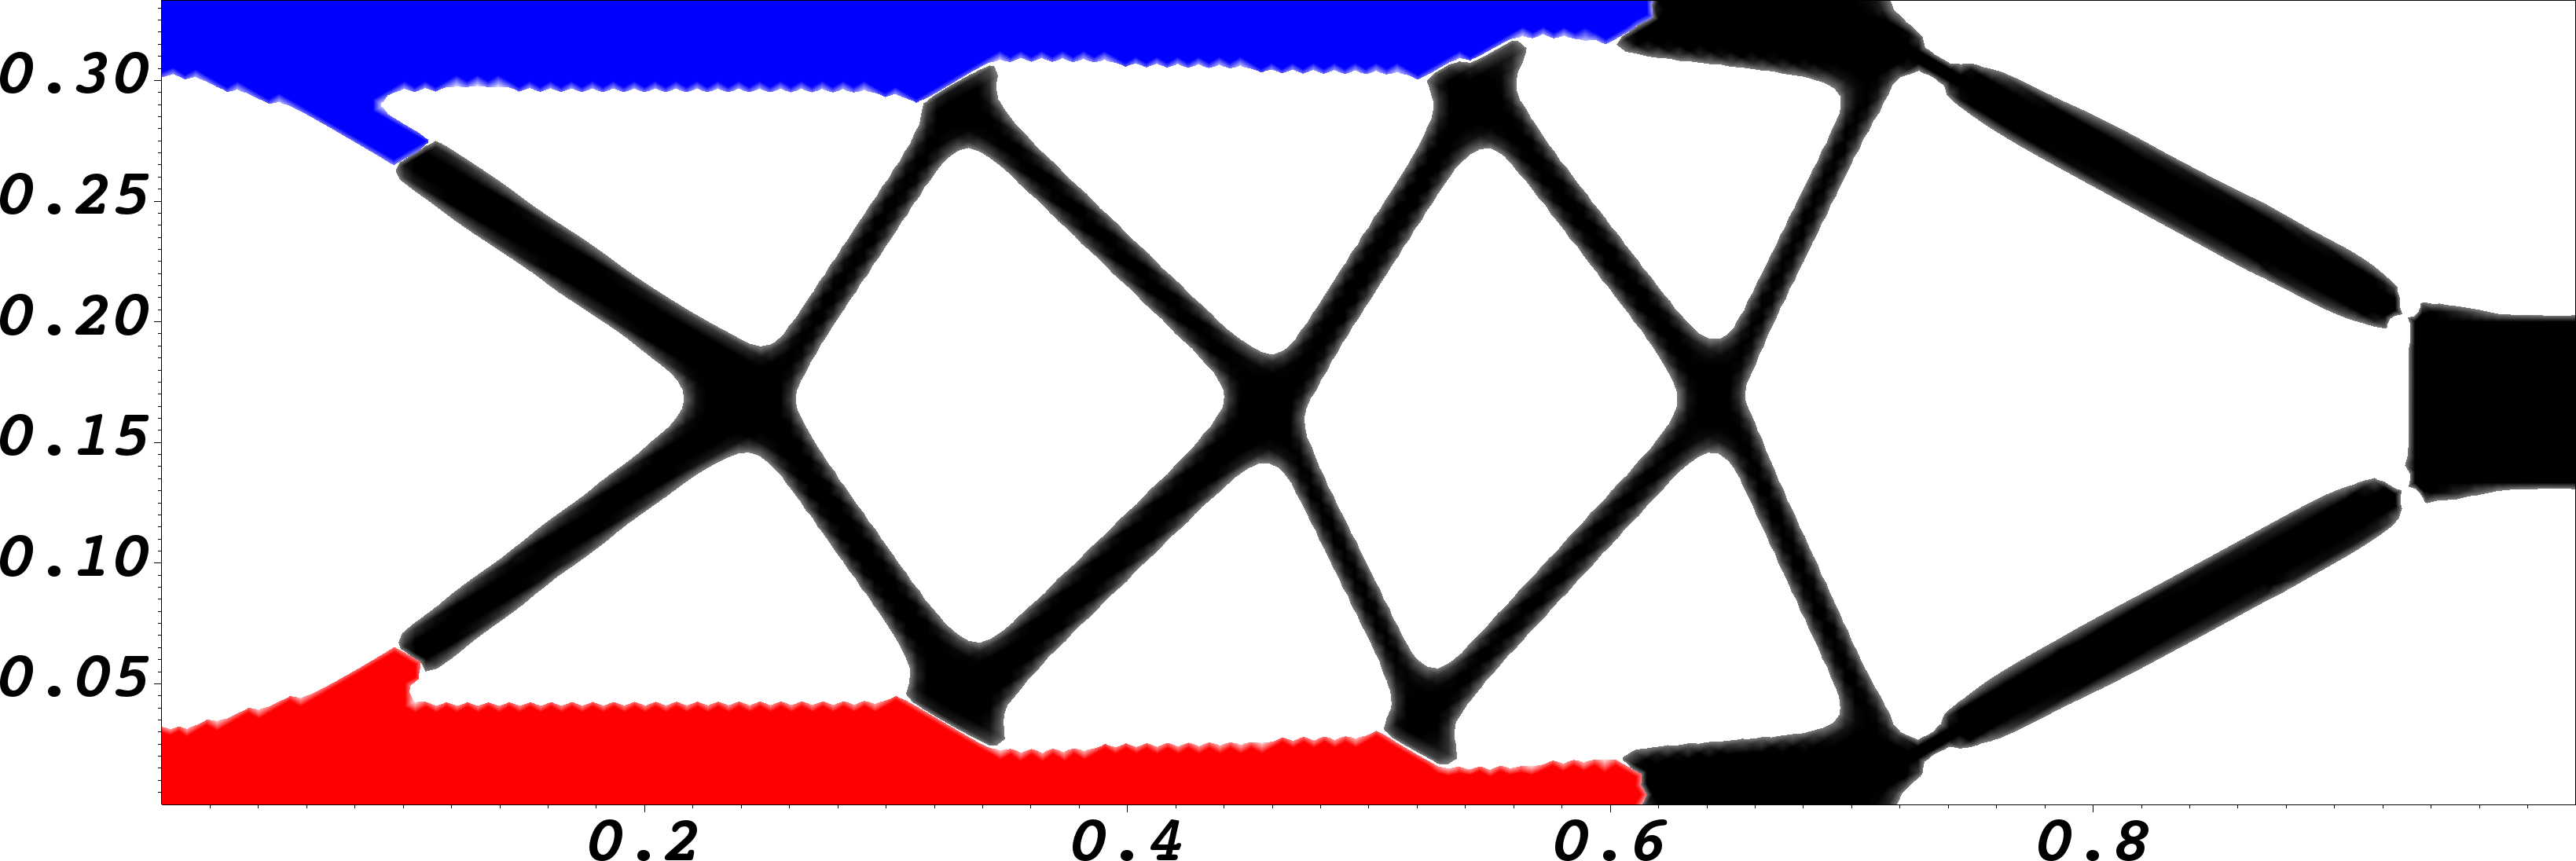
\includegraphics[width=0.45\textwidth]{figures/BeamLoadRatio1DirLS-Composite.png}\par
            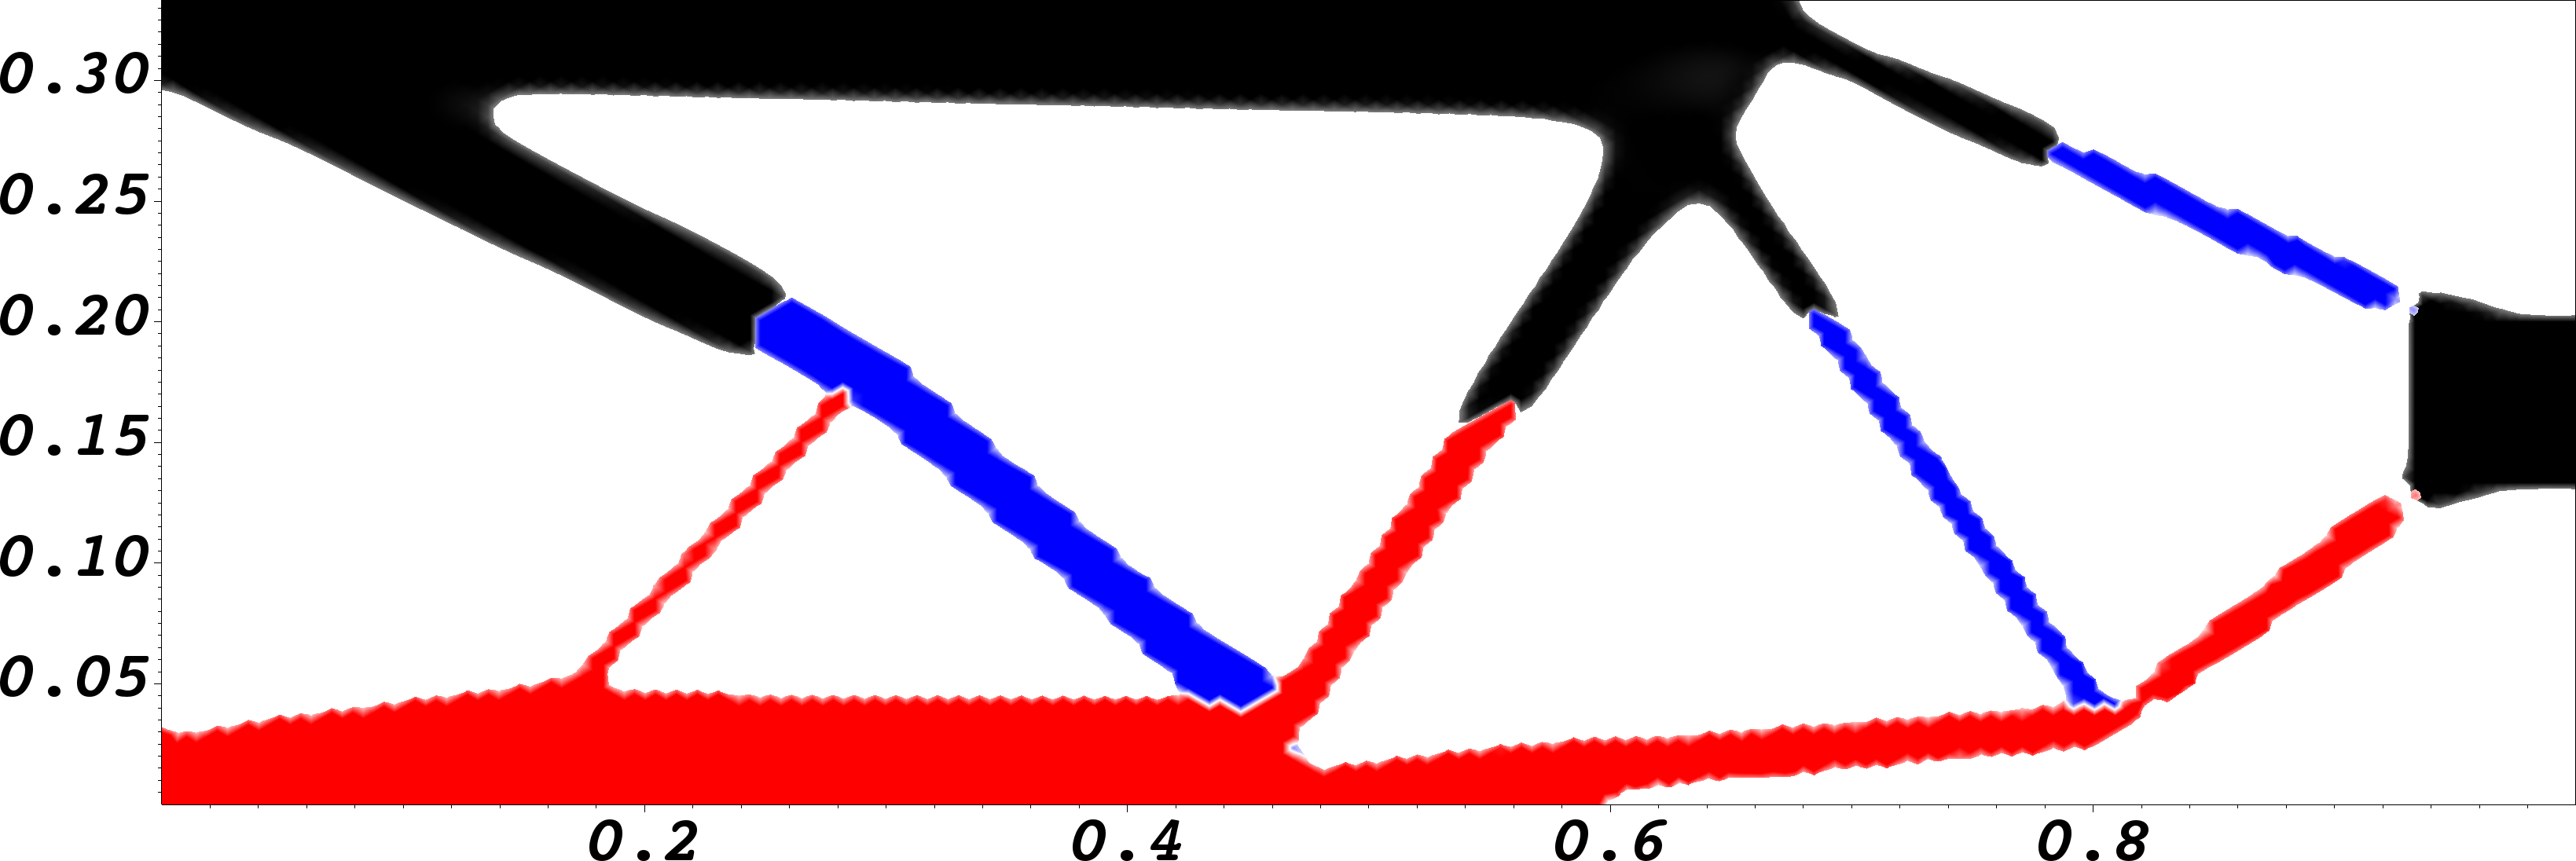
\includegraphics[width=0.45\textwidth]{figures/BeamLoadRatio1DirLS-Composite2.png}\par
        \end{multicols}
        \begin{multicols}{2}
            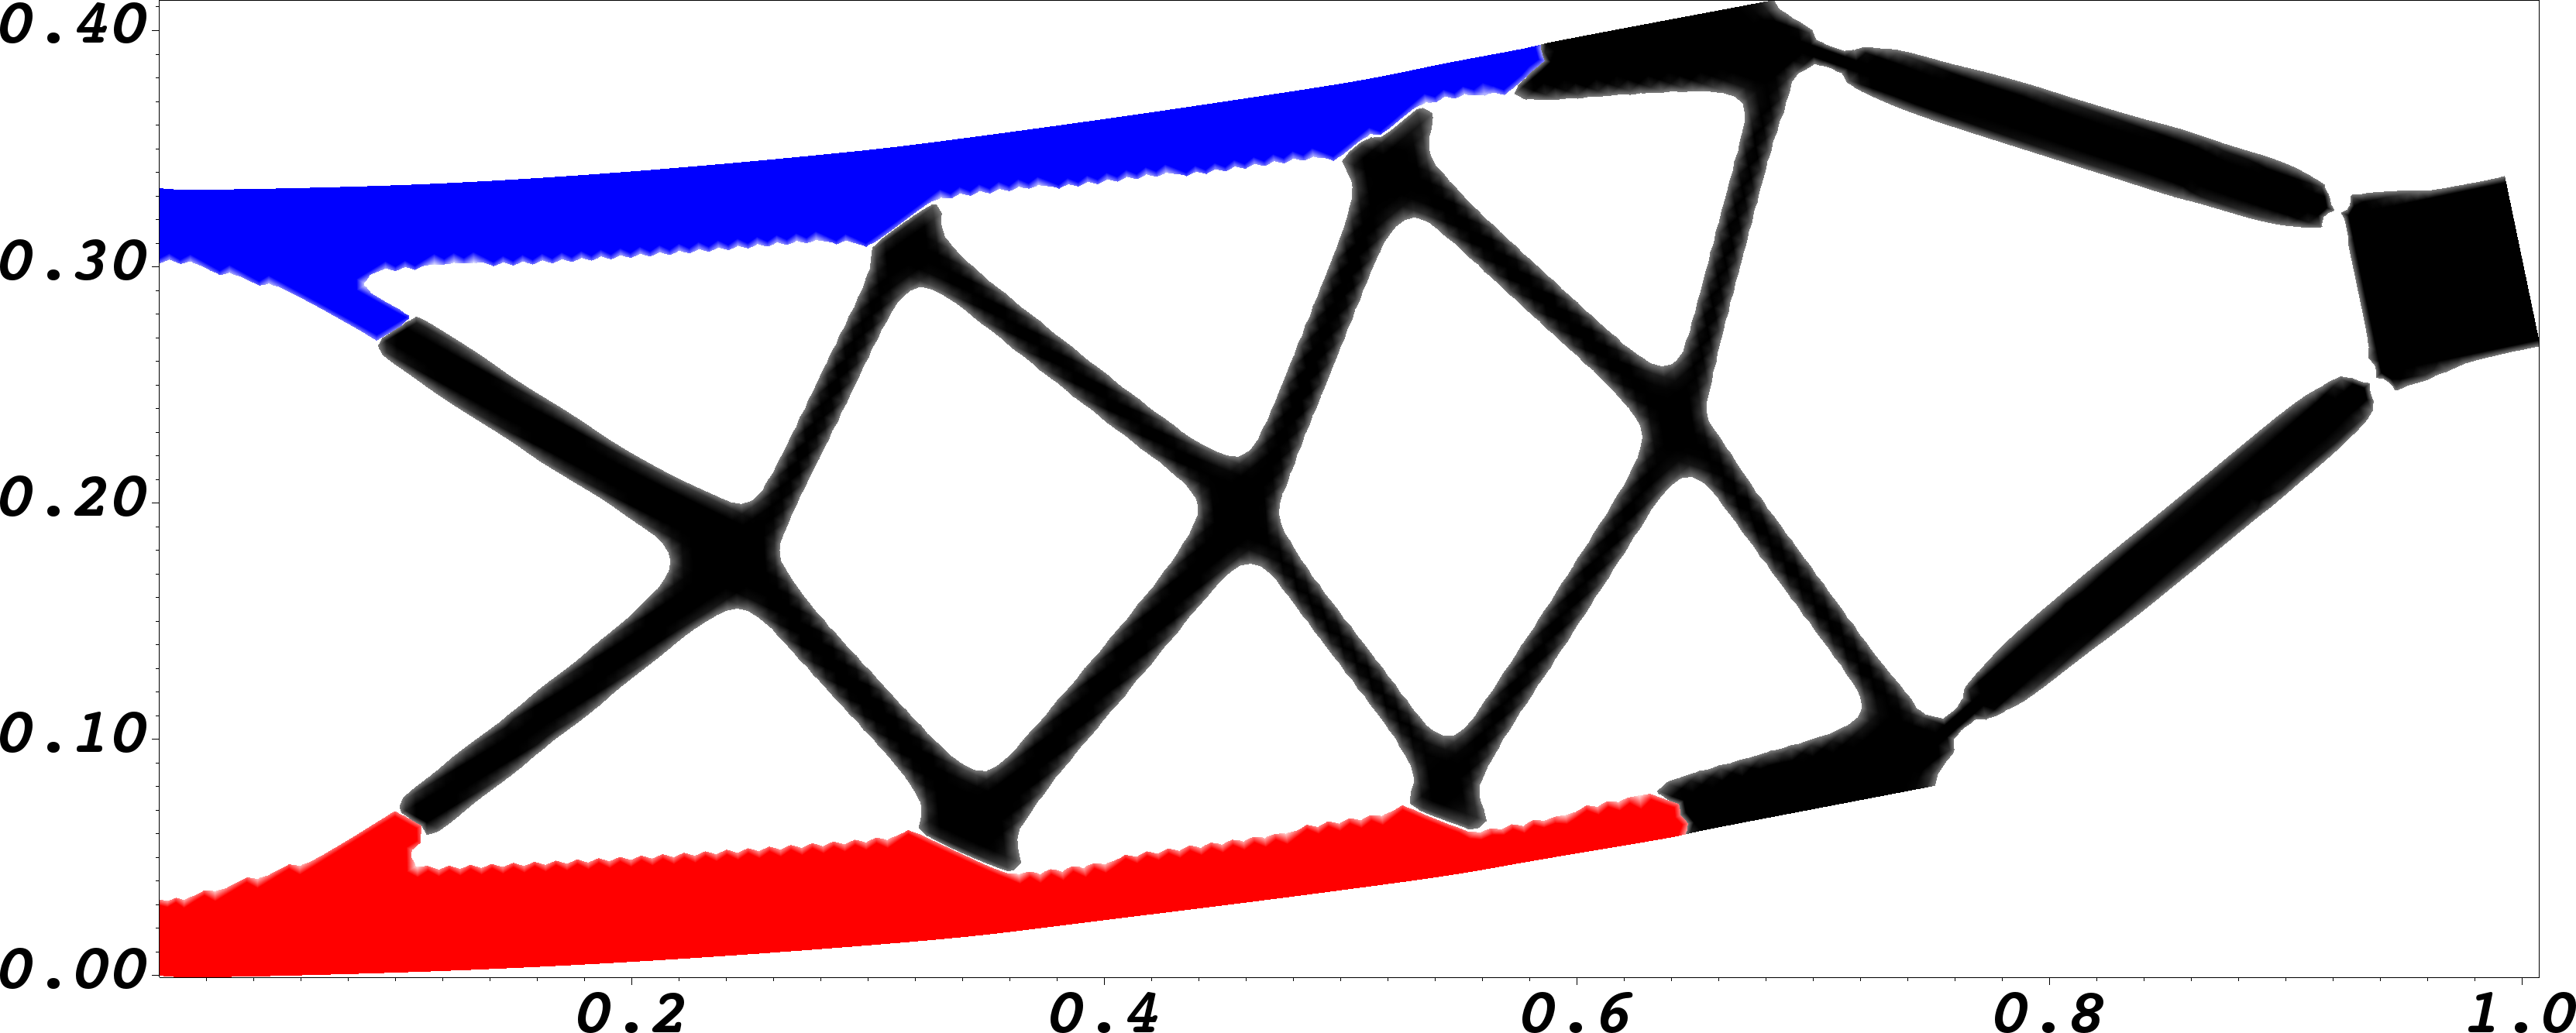
\includegraphics[width=0.45\textwidth]{figures/BeamLoadRatio1DirLS-disp.png}\par
            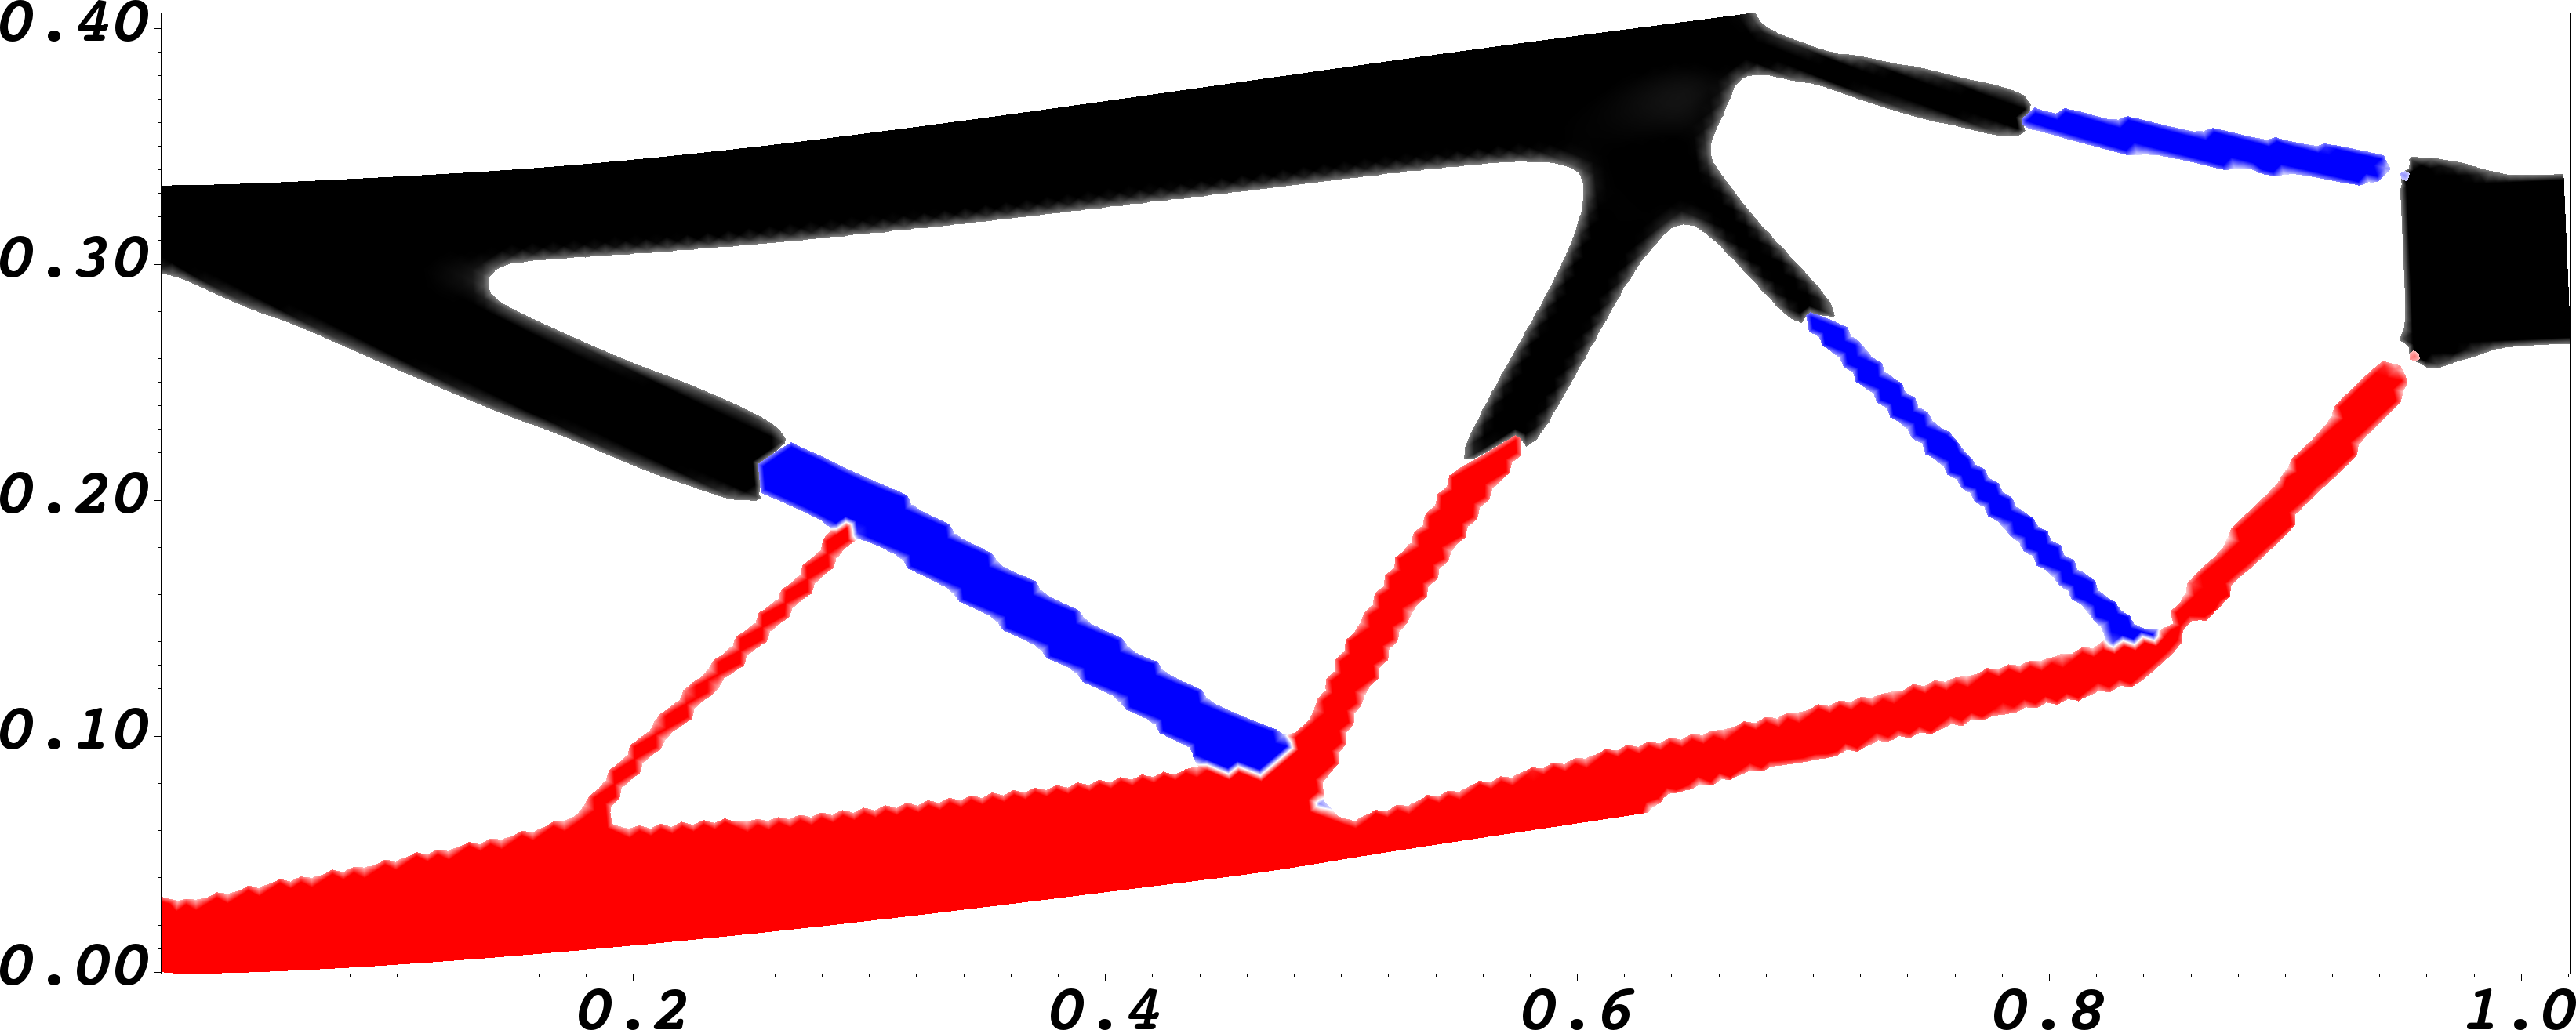
\includegraphics[width=0.45\textwidth]{figures/BeamLoadRatio1DirLS-disp2.png}\par
        \end{multicols}
        \begin{multicols}{2}
            \centering
            $\text{Objective function}=4.17 \times 10^{-3}$\\
            $\text{Objective function}=4.49 \times 10^{-1}$
        \end{multicols}
        \caption{Staggered (left) vs. Monolithic (right) approach. Composite plot 
        of both material density and the stimulus in the reference (top) and deformed (bottom) configuration for stiffness ratio $E_3/E_2=1.0$.}
        \label{fig:schemeComparison}
    \end{figure}
\end{frame}

\section{Responsive optimal design with stimulus as a state variable}
\subsection{Stimulus governed by poisson PDE}
\begin{frame}{Stimulus governed by poisson PDE}
    \begin{itemize}
        \item Let the design variable $\tp=[\p_s,\p_r,g]^T.$
        \item $g \in [-1,1]$ is the stimulus control function.
        \item The problem can be stated as:
            \begin{equation*}
                \begin{dcases}
                \begin{aligned}
                    &\min_{(\p,g)}\;\; \frac{1}{2}\int_{\OO_0}|u-\bar{u}|^2\;dx + \alpha\PP_{\e}(\tp,s) + Q(\tp,g) + V_C(\tp)\\
                    &u \text{ and }s\text{ satisfy the weak forms }(\ref{eq:statePFWeak2})\text{ and }(\ref{eq:statePoisson})
                \end{aligned}
                \end{dcases}
            \end{equation*}
            \begin{equation}
                \label{eq:statePFWeak2}
                \sum_{i=\{v,s,r\}}\int_\OO a(\p_i)\mathbb{C}_i\left(\ee(u)-\beta_i s\mathrm{I}_d\right)\cdot \ee(v)\, dx = 0\ \forall v \in V,
            \end{equation}
            \begin{equation}\label{eq:statePoisson}
                \sum_{i=\{v,s,r\}}\int_\OO k(\p_i)\nabla s \cdot \nabla q\,dx - \int_{\OO}gq\,dx = 0
            \end{equation}
    \end{itemize}
\end{frame}

\begin{frame}{Stimulus governed by poisson PDE}
    \begin{itemize}
        \item Target displacement $\bar{u}=(0,1).$
    \end{itemize}
    \begin{figure}[H]
        \centering
        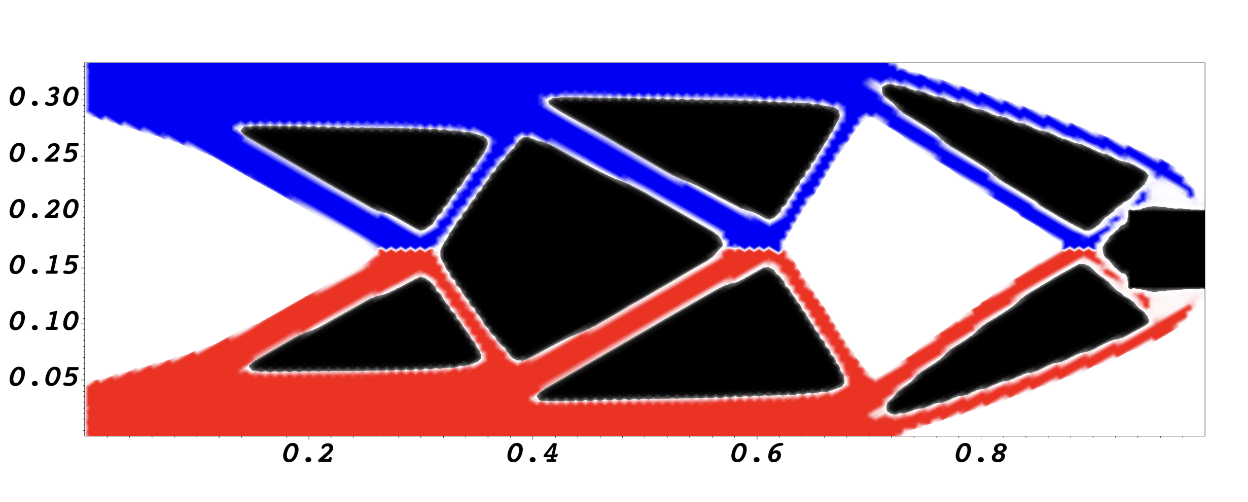
\includegraphics[width=0.45\textwidth]{figures/BeamLoadRatio100DirLS-Composite.png}
        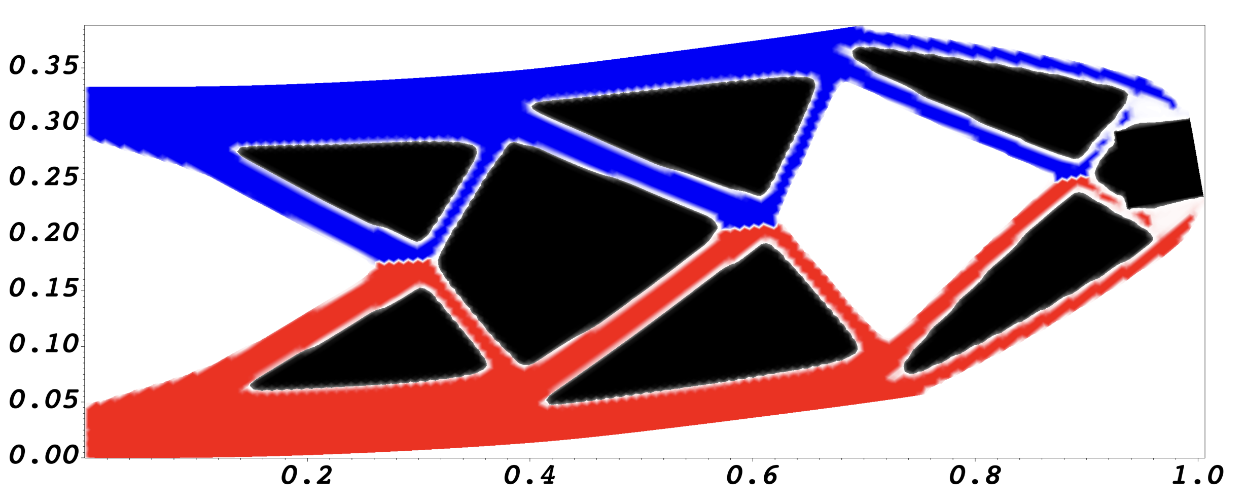
\includegraphics[width=0.45\textwidth]{figures/BeamLoadRatio100DirLS-disp.png}
        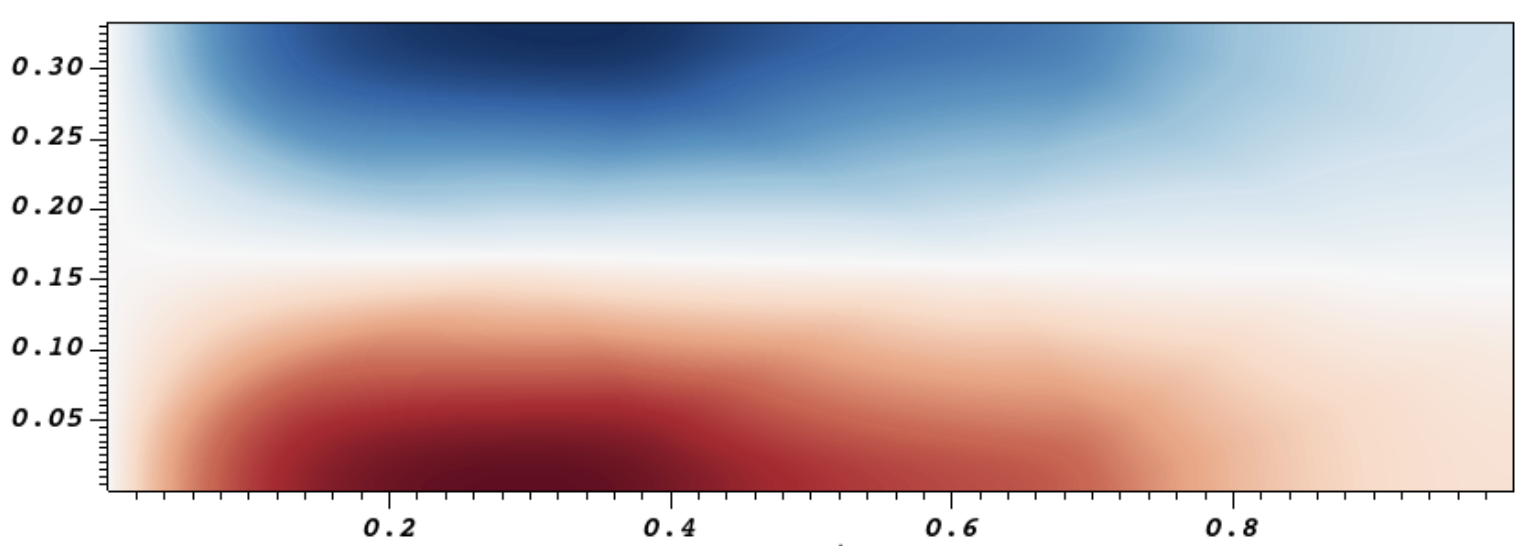
\includegraphics[width=0.5\textwidth]{figures/stimulus.png}
        \caption{Composite plot of both material density and the heat source in 
        the reference (top) and deformed configuration (bottom) for stiffness 
        ratio $E_3/E_2=100.$ The red and blue represent the area of the responsive 
        material with heat source values $1$ and $-1$ respectively.}
        \label{fig:designs-staticRatio10}
    \end{figure}
\end{frame}
%%%%%%%%% End of SECTION 3 %%%%%%%

%%%%%%%%% Begin of SECTION 4 %%%%%%%
\section{Conclusion}
\begin{frame}{Conclusion}
    \begin{itemize}
        \item Responsive optimal design
        \bigskip
        \item Responsive optimal design with stimulus as a design variable
        \bigskip
        \begin{itemize}
            \item Least square objective function with $n$ target displacements
            \item A paper was submitted titled "Systematic design of compliant morphing
            structures: a phase-field approach".
        \end{itemize}
        \bigskip
        \item Responsive optimal design with stimulus as a state variable
        \bigskip
        \begin{itemize}
            \item Stimulus governed by Poisson PDE
            \bigskip
        \end{itemize}
        \item Stimulus governed by Transient heat PDE (\bf Show some animations.)
    \end{itemize}
\end{frame}

\begin{frame}[shrink=40]{References} 
    \bibliography{defence}
    \bibliographystyle{ieeetr}
    \nocite{*}
\end{frame}
%%%%%%%%% End of SECTION 4 %%%%%%%

\begin{frame}
\Huge{\centerline{Thank You!}}
\end{frame}
\end{document}